\documentclass[a4paper,14pt]{article}
\usepackage{float}
\usepackage{extsizes}
\usepackage{amsmath}
\usepackage{amssymb}
\everymath{\displaystyle}
\usepackage{geometry}
\usepackage{fancyhdr}
\usepackage{multicol}
\usepackage{graphicx}
\usepackage[brazil]{babel}
\usepackage[shortlabels]{enumitem}
\usepackage{cancel}
\columnsep=2cm
\hoffset=0cm
\textwidth=8cm
\setlength{\columnseprule}{.1pt}
\setlength{\columnsep}{2cm}
\renewcommand{\headrulewidth}{0pt}
\geometry{top=1in, bottom=1in, left=0.7in, right=0.5in}

\pagestyle{fancy}
\fancyhf{}
\fancyfoot[C]{\thepage}

\begin{document}
	
	\noindent\textbf{1MMA01~Matemática} 
	
	\begin{center}Ideias iniciais sobre ângulos e polígonos (Versão estudante)
	\end{center}
	
	\noindent\textbf{Nome:} \underline{\hspace{10cm}}
	\noindent\textbf{Data:} \underline{\hspace{4cm}}
	
	%\section*{Questões de Matemática}
	
    \begin{multicols}{2}
    	Primeira parte - conceitos iniciais 
    	\begin{enumerate}
    		\item Desenhe e defina (de forma resumida) os ângulos indicados abaixo. 
    		\begin{enumerate}[a)]
    			\item Ângulo agudo \\\\\\\\\\\\\\
    			\item Ângulo reto \\\\\\\\\\\\\\
    			\item Ângulo obtuso \\\\\\\\\\\\\\
    		\end{enumerate}
    	    \item O que você entende por: 
    	    \begin{enumerate}[a)]
    	    	\item Ângulos complementares:  \\\\\\
    	    	\item Ângulos suplementares:  \\\\\\
    	    	\item Ângulos opostos pelo vértice:  \\\\\\
    	    \end{enumerate}
		        Vamos continuar nossa revisão? 
		        
		        Agora, vamos utilizar a ideia de ângulo para classificar triângulos e quadriláteros 
		        
		        \item Como você já sabe, todo triângulo possui três lados e três ângulos. Com relação aos ângulos, teremos três tipos de triângulos:
        
	        \begin{enumerate}[a)]
	        	\item Acutângulo \\\\\\\\
	        	\item Obtusângulo \\\\\\\\
	        	\item Retângulo \\\\\\\\
	        \end{enumerate}
		        Como você diferencia cada um deles? Explique resumidamente. \\\\\\\\\\\\\\\\\\
		        No que se refere aos quadriláteros, podem ser agrupados com relação aos lados da seguinte maneira:
            \begin{enumerate}[a)]
            	\item Paralelogramos \\
            	(Possuem dois pares de lados paralelos) \\ 
            	$\begin{cases}
            		\text{Retângulo} \\
            		\text{Losango} \\
            		\text{Quadrado} \\
            		\text{Outros}
            	\end{cases}$
            	\item Trapézios \\
            	(Possuem um par de lados paralelos) \\
            	$\begin{cases}
            		\text{Escaleno} \\
            		\text{Retângulo} \\
            		\text{Isósceles}
            	\end{cases}$
            	\item Trapezóides \\
            	(Não possuem pares de lados paralelos)
            \end{enumerate}
        	\item Com relação aos ângulos, como você agrupa estes quadriláteros? Ou seja, como separar estes quadriláteros considerando os seus ângulos internos? \\\\\\\\\\\\\\\\\\\\\\
        	Segunda parte - resolução de questões 
        	\item O relógio a seguir marca 9h:
        	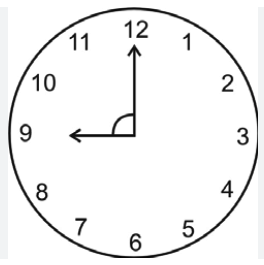
\includegraphics[width=1\linewidth]{1MMA01_imagens/imagem01}
        	Assinale a alternativa que mostra corretamente qual a medida do ângulo formado pelos dois ponteiros indicado na figura. \\\\
        	a) 180$^\circ$
        	
        	b) 90$^\circ$
        	
        	c) 60$^\circ$
        	
        	d) 45$^\circ$
        	
        	\item Lourenço estava com seu skate posicionado para a esquerda, como mostra a figura 1, e a seguir fez uma manobra dando um giro de forma posicionar o skate para a direita, como mostra a figura 2.
        	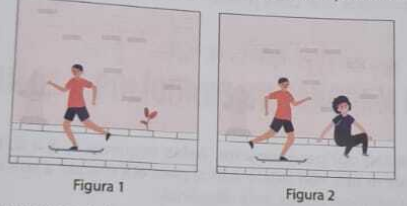
\includegraphics[width=1\linewidth]{1MMA01_imagens/imagem02}
        	Medida de ângulo que pode ser associada ao giro dessa manobra é \\\\
        	a) 45$^\circ$
        	
        	b) 90$^\circ$
        	
        	c) 180$^\circ$
        	
        	d) 360$^\circ$ 
        	
        	\item A imagem apresentada a seguir é uma representação da tela quadrada intitulada O peixe, de Marcos Pinto, que foi colocado em uma parede para exposição e fixadas nos pontos A e B. Por um problema na fixação de um dos pontos, a tela se desprendeu girando rente à parede. Após o giro, ela ficou posicionada como ilustrado na figura formando um ângulo de 45$^\circ$  com a linha do horizonte. \\\\
        	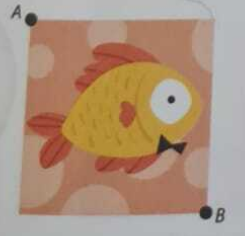
\includegraphics[width=1\linewidth]{1MMA01_imagens/imagem03}
        	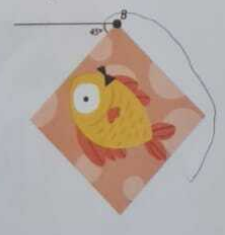
\includegraphics[width=1\linewidth]{1MMA01_imagens/imagem04}
        	Para recolocar a tela na sua posição original, deve-se girá-la, rente à parede no menor ângulo possível inferior a 360$^\circ$. \\
        	A forma de recolocar a tela na posição original, obedecendo ao que foi estabelecido, é girando-a em um ângulo de 
        	\\\\
        	a) 90$^\circ$ no sentido horário 
        	
        	b) 135$^\circ$ no sentido horário 
        	
        	c) 180$^\circ$ no sentido anti-horário 
        	
        	d) 270$^\circ$ no sentido anti-horário 
        	
        	e) 315$^\circ$ no sentido horário
        	
        	\item Para chegar a sua casa Lídia tem que seguir o trajeto representado na malha a seguir passando pelas esquinas 1,2 e 3. Para fazer isso você pode adicionar três comandos: avançar (indicando o número de lados do quadradinho), virar à direita e virar à esquerda. \\
        	Indique a sequência de comandos que Lídia precisará fazer para chegar em sua casa.
        	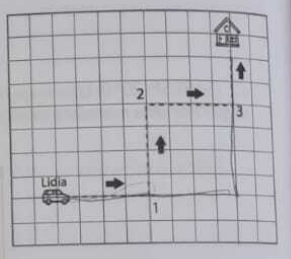
\includegraphics[width=1\linewidth]{1MMA01_imagens/imagem05}\\\\\\\\\\\\\\
        	Se, Lídia não precisasse passar, obrigatoriamente, pelas esquinas 1, 2 e 3, teria outro trajeto mais curto? Indique outro caminho (mesmo que não seja o curto) para ela chegar a sua casa. (Todos os trajetos devem passar por lados dos quadradinhos, nunca pela diagonal.)\\\\\\\\
        	\item Qual a medida dos dois ângulos formados pelos ponteiros de um relógio às 8 horas?\\
        	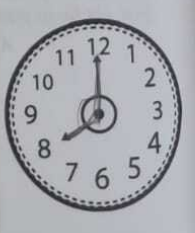
\includegraphics[width=1\linewidth]{1MMA01_imagens/imagem06}\\\\\\\\
        	\item Observe a figura abaixo:
        	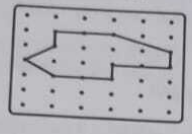
\includegraphics[width=1\linewidth]{1MMA01_imagens/imagem07}
        	Desenhe na malha pontilhada abaixo a figura acima após realizarmos um giro de 90 graus no sentido horário.
        	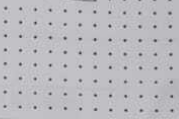
\includegraphics[width=1\linewidth]{1MMA01_imagens/imagem08}
    	\end{enumerate}
	\end{multicols}
\end{document}